\documentclass{article}
\usepackage{graphicx}
\usepackage{subcaption}
\usepackage{amsmath}
\usepackage{float}

\title{Homework 3 Question 2}
\author{Mudit Sethia, Yash Rampuria, Disha Pandey}
\date{\today}

\begin{document}

\maketitle

\section{Introduction}
In this assignment, we implemented two types of low pass filters, namely the ideal low pass filter and the Gaussian low pass filter, with different cutoff frequencies and standard deviations, respectively. We applied these filters to the "barbara256.png" image and analyzed their effects. Additionally, we examined the frequency responses of these filters and the Fourier transforms of the original and filtered images.

\section{Implementation}

\subsection{Reading and Preprocessing the Image}
We started by reading the "barbara256.png" image and converting it to a double precision format. The original image was displayed for reference. To ensure proper filtering, we padded the image to double its dimensions.

\subsection{Ideal Low Pass Filter}
For the ideal low pass filter, we implemented the \texttt{IdealLowPass} function. This function computes the Fourier transform of the input image, creates a filter with a specified cutoff frequency, and applies the filter in the frequency domain. The resulting image was obtained by performing the inverse Fourier transform.

\subsection{Gaussian Low Pass Filter}
Similarly, we implemented the \texttt{GaussianLowPass} function for the Gaussian low pass filter. This function applies a Gaussian filter to the Fourier transform of the input image based on a given standard deviation (\(\sigma\)). The inverse Fourier transform yields the filtered image.

\section{Results}

\subsection{Ideal Low Pass Filter Results}
We applied the ideal low pass filter with two different cutoff frequencies, \(D = 40\) and \(D = 80\). Figure \ref{fig:ideal_results} shows the filtered images for both cutoff frequencies.

\begin{figure}[H]
    \centering
        \centering
        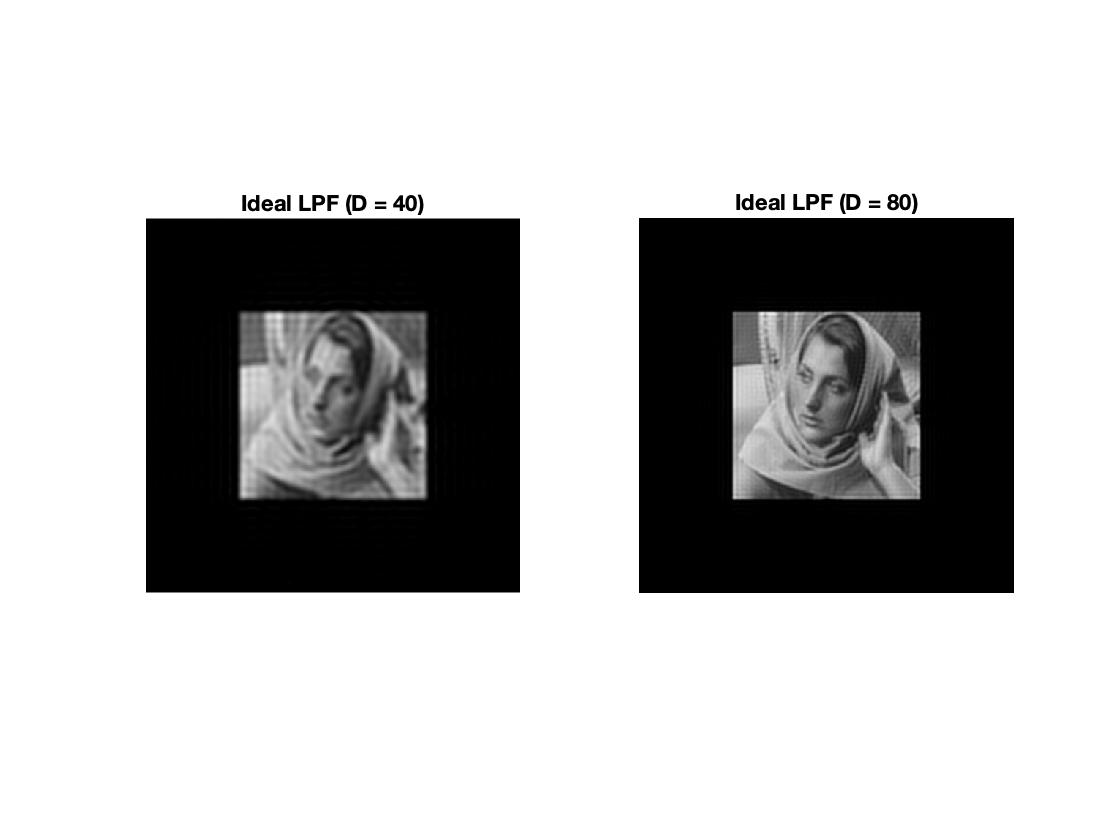
\includegraphics[width=\linewidth]{Ideal_Low_Pass.png}
        \caption{Ideal LPF}
    
\end{figure}

\subsection{Gaussian Low Pass Filter Results}
We also applied the Gaussian low pass filter with two different standard deviations, \(\sigma = 40\) and \(\sigma = 80\). Figure \ref{fig:gaussian_results} presents the filtered images for these two \(\sigma\) values.

\begin{figure}[H]
    \centering
        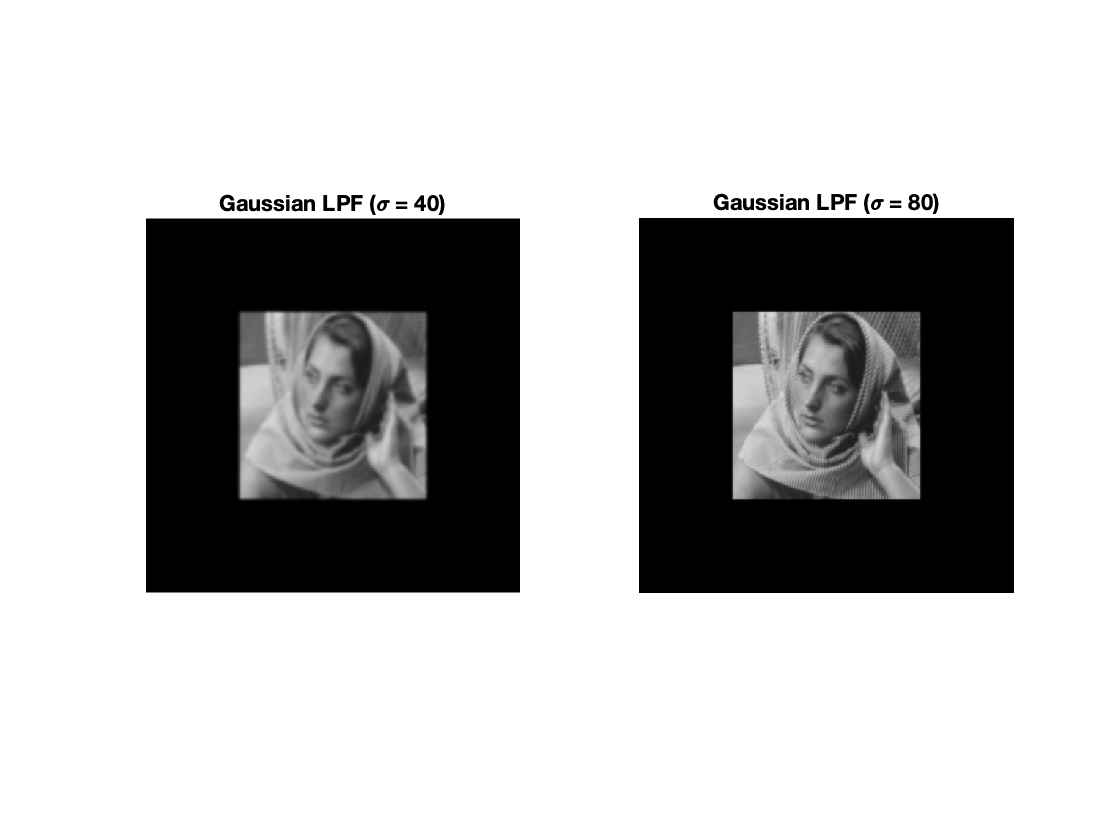
\includegraphics[width=\linewidth]{Gaussian_Low_Pass.png}
        \caption{Gaussian LPF}
\end{figure}

\subsection{Frequency Response and Fourier Transforms}
To analyze the frequency response of the filters and the Fourier transforms of the images, we calculated and displayed the log absolute Fourier transforms. Figure \ref{fig:frequency_response} shows the frequency responses of the filters, and Figure \ref{fig:fourier_transforms} presents the Fourier transforms of the original and filtered images.

\begin{figure}[H]
    \centering
        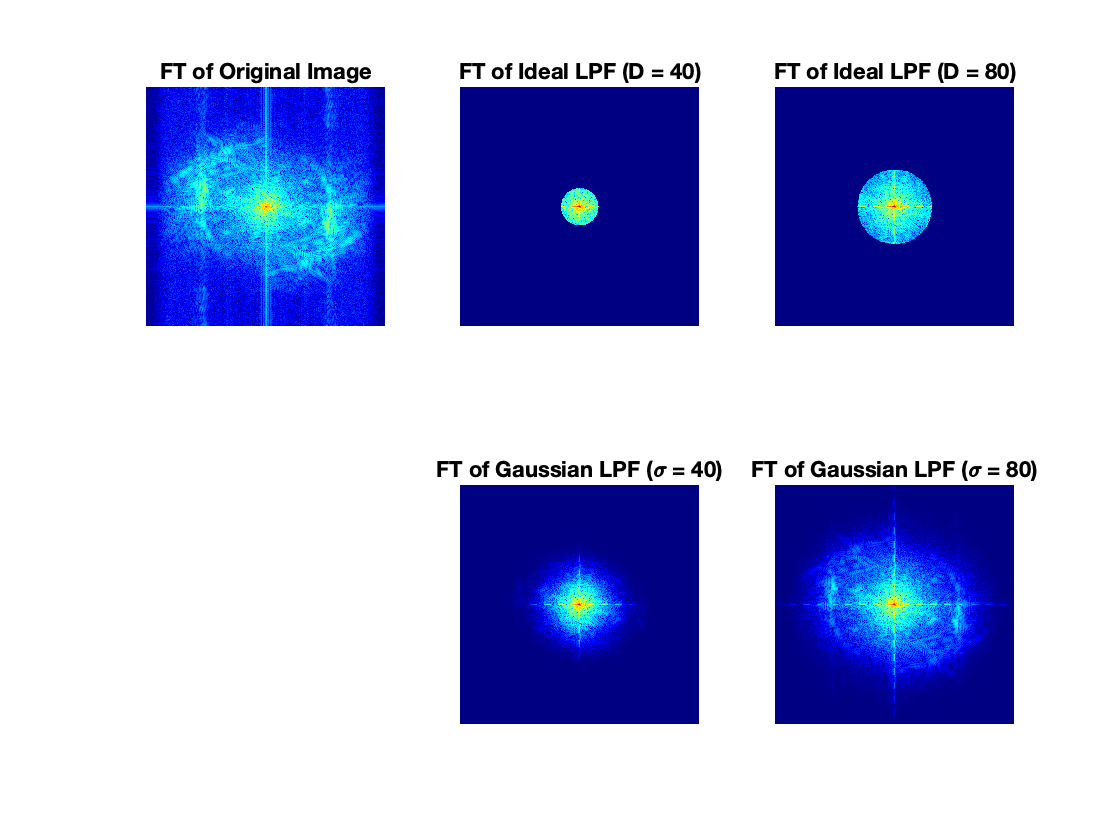
\includegraphics[width=\linewidth]{Fourier_Transforms_All.png}
        \caption{Frequency Response and Fourier Transforms}
\end{figure}

\section{Discussion}

In this section, provide a detailed analysis of the differences in the filtered images, frequency responses, and Fourier transforms. Comment on the impact of changing cutoff frequencies and standard deviations on the filtering results and the characteristics of the filters.

\section{Conclusion}

Summarize the key findings of your analysis and the overall impact of the different filters on the image.

\end{document}
